\begin{figure}[tbh]
    \centering
    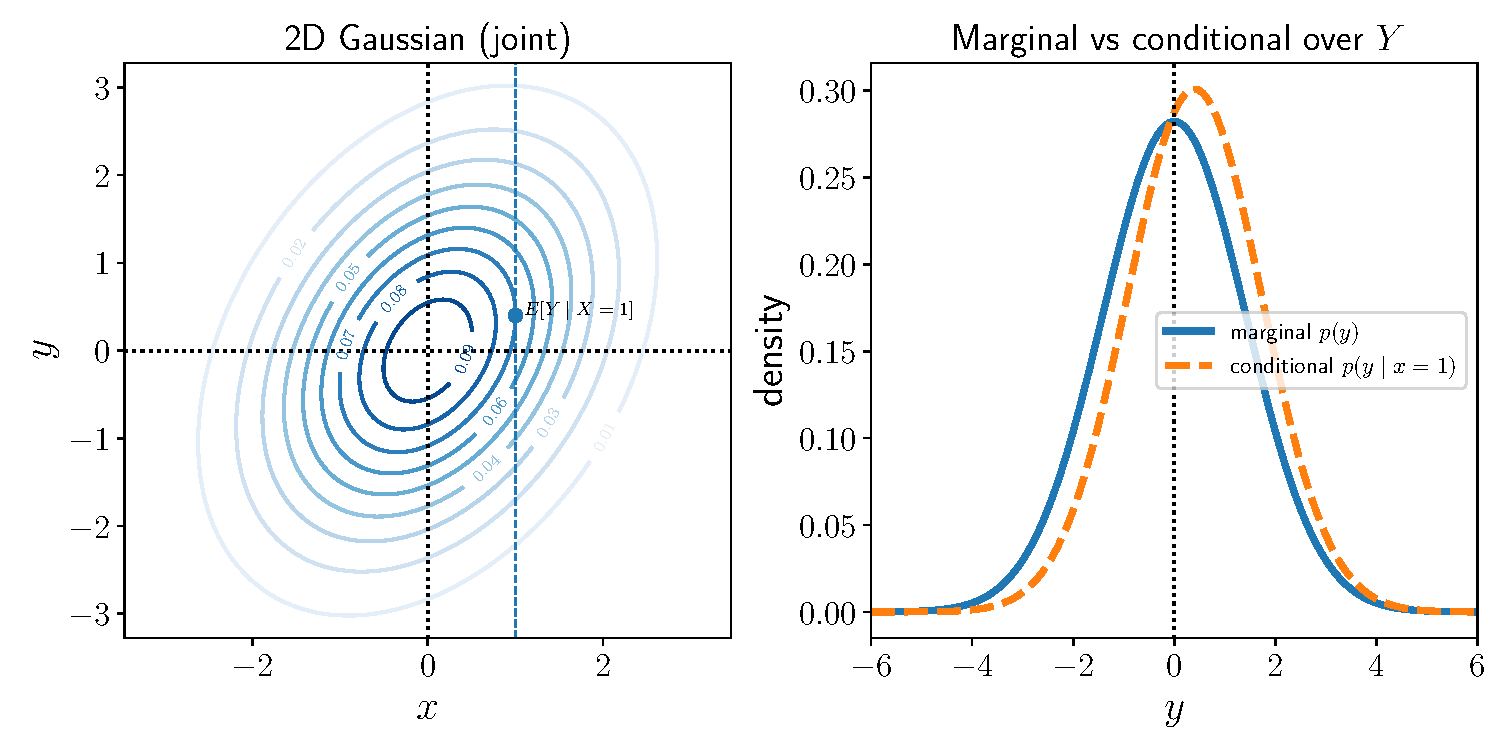
\includegraphics[width=0.8\linewidth]{2D_Gaussian_demo.pdf}
    \caption{(Left) Contour plot illustrating the shape of the joint probability distribution function of a two-dimensional Gaussian $p(x,y)=\mathcal{N}(\bm{\mu},\bm{\Sigma})$ with mean at the origin and a covariance matrix of non-zero off-diagonal elements.  (Right) Showing the corresponding one-dimensional conditional distribution $p(y|x=1)$ (blue dashed line on the left figure, the blue dot on which indicates the conditional mean $\mathbb{E}[y|x=1]$) and the marginal distribution $p(y)$ that is marginalised over $x$ which is centred at $y=0$. }
    \label{fig:2D_Gaussian_demo}
\end{figure}

In reality, the physical behaviours of a system often depend on multiple (multidimensional) random variables $\{\bm{x}_1,\bm{x}_2,\ldots,\bm{x}_n\}$, such as the total energy of an atomistic system expressed in terms of the three-dimensional Cartesian coordinates of each constituent atoms $E(\bm{R}_1,\bm{R}_2,\ldots,\bm{R}_n)$. In this case, the probability that a system will take a particular state is described by the \textit{joint probability distribution} $p(\bm{x}_1,\bm{x}_2,\cdots\bm{x}_n)$, which is the probability that all the random variables will simultaneously fall into a set of given values [see \cref{fig:2D_Gaussian_demo}(left) for an illustration for a simple two-dimensional joint Gaussian distribution].  For atomistic systems, local minima on the PES correspond to local maxima of the joint probability distribution. It is also a common case, that for a system described by the joint probability distribution   $p(\bm{x}_1,\bm{x}_2,\cdots,\bm{x}_n)$, the value that each variable $\bm{x}_i$ will take is no longer independent by become highly correlated with the values of other variables $\{\bm{x}_j|j\neq i\}$. For instance, the distributions of dihedral angles in a polypeptide is highly correlated in order to avoid stereo-hinderance, which is commonly demonstrated by the Ramachandran plot. \cref{fig:2D_Gaussian_demo}(left) shows this behaviour with a 2D Gaussian that is not symmetric with respect to either the $x$- or $y$-axis, for which the variance is described by a matrix $\bm{\Sigma}$ where its diagonal element corresponds to the variance in the $i$-th dimension $\mbox{Var}[\bm{x}_i]$, and the off-diagonal element corresponds to the \emph{covariance}  $\mbox{Cov}[\bm{x}_i,\bm{x}_j]=\mathbb{E}\Big[[\bm{x}_i-\mathbb{E}[\bm{x}_i]][\bm{x}_j-\mathbb{E}[\bm{x}_j]]\Big]$ that measures the degree of correlation between the $i$- and $j$-th random variables. Physically, it is conceptually similar to quantities such as the off-diagonal terms in the force-constant matrix [\cref{eq:FC_finite_difference}] which reflects how strongly the simultaneous perturbation on two atomic positions will shift the system energy.\footnote{To see this, we take the harmonic approximation to the local PES as $E(\bm{x})=\frac{1}{2}\bm{x}^\top \bm{\Phi}\bm{x}$, such that under the canonical ensemble, the corresponding probability distribution function for the atomic displacements follows $p(\bm{x})=\exp(-\beta \bm{x}^\top \bm{\Phi}\bm{x}/2)$, which is a normal distribution with its covariance matrix being $\bm{\Sigma}=\bm{\Phi}^{-1}/\beta$. This shows that the covariance matrix of fluctuations in the atomic displacements is proportional to the inverse of the Hessian. More specifically, we have $\bm{\Sigma}(i,j)=\bm{\Phi}_{ij}^{-1}/\beta$, thus demonstrating the off-diagonal elements for the force-constant matrix is related to the covariance of the probability distribution.}

Directly working with high-dimensional joint probability distributions is often intractable. This can be solved by dealing with subsets of the joint probability distributions, for which the two concepts that are most relevant here are the conditional and marginal probability distributions [\cref{fig:2D_Gaussian_demo}(right)]. The conditional probability  $p(\bm{x}|\bm{\theta})$ describes the probability of occurrence for a particular event $\bm{x}$ when some other variables or parameters that might affect the shape of the probability distribution function is fixed at a specific choice $\bm{\theta}$. This gives us the language to formulate the probabilistic equivalent to forcefield training [\cref{eq:FF_fitting}] for training the ML/AI model, which is a process of optimising the parameters $\bm{\theta}$ until the conditional probability distribution $p_{\mbox{\scriptsize{tr}}}(\bm{x}|\bm{\theta})$ described by the model reaches the best match to the target distribution $p_{\mbox{\scriptsize{target}}}(\bm{x})$, and we shall further consolidate this idea in the subsequent discussions. Fundamentally, the joint  and conditional distributions are related as:
\begin{equation}
    \label{eq:joint_cond_prob}
p(\bm{x}_1,\bm{x}_2,\ldots,\bm{x}_n)=p(\bm{x}_1)\prod_{i=2}^n p(\bm{x}_i|\bm{x}_{i-1}).
\end{equation}
The marginal probability, on the other hand, is the probability distribution over a subset of random variables with the rest of the random variables being integrated out, \emph{e.g.}
\begin{equation}
    \label{eq:marginal_distribution}
    p_{X}(\bm{x})=\int p_{X,Y}(\bm{x},\bm{y})\mbox{d}\bm{y}.
\end{equation}
This follows that
\begin{equation*}
    p_{Y|X}(\bm{y}|\bm{x})=\frac{p_{X,Y}(\bm{x}|\bm{y})}{p(\bm{x})},
\end{equation*}
which is an expression that is most commonly used in the \textbf{\textit{Bayes' rule}} underpinning the modern probabilistic interpretations of ML/AI:
\begin{equation}
    \label{eq:bayes_rule}
    p(\bm{y}|\bm{x})=\frac{p(\bm{x}|\bm{y})p(\bm{y})}{p(\bm{x})}.
\end{equation}
For example, during training of an ML/AI model, one typically starts by initialising the model with a set of parameters $\mathbf{\theta}$ that are drawn from some prior belief on their values $p(\mathbf{\theta})$, and the likelihood that that training data $\bm{x}$ will be observed under these parameters is given by the conditional distribution $p(\bm{x}|\theta)$. After the model observed the training data given, the posterior probability distributions for the parameters will be updated according to \cref{eq:bayes_rule} as $p(\theta|\bm{x})=p(\bm{x}|\theta)p(\theta)/p(\bm{x})$, whereby parameters drawn from this updated distributions will lead to a model with better performance of predicting the outcome on the training data $\bm{x}$.
